\documentclass[10pt, a4paper]{scrartcl}

\usepackage{vorschule}
\usepackage[
	typ=ab,
	fach=Informatik,
	lerngruppe={Q2-GK},
	nummer=II.5,
	module={Symbole,Lizenzen},
	seitenzahlen=keine,
	farbig,
	lizenz=cc-by-nc-sa-4,
]{schule}

\usepackage[
	kuerzel=Ngb,
	reihe={Rechnernetze},
	version={2020-11-20},
]{ngbschule}

\author{J. Neugebauer}
\title{Telnet}
\date{\Heute}

\setzeAufgabentemplate{ngbnormal}

\begin{document}
\ReiheTitel

Ein \emph{Telnet-Client} ist ein Programm, mit dem Verbindungen zu Servern hergestellt werden können. Auf fast jedem Betriebssystem gibt es einen \emph{Telnet-Client}. Unter Windows startet man zum Beispiel eine Kommandozeile (\appfunktion{Start} $\rightarrow$ \code{cmd} $\rightarrow$ \taste{ENTER}) und gibt den Befehl \code{telnet} gefolgt von einer \emph{IP-Adresse} oder einem \emph{Hostnamen} und einer \emph{Portnummer} ein. Telnet kommuniziert also über eine \emph{TCP-Verbindung}.

Um zum Beispiel eine Verbindung zum Google-Server über den Port 80 (HTTP) aufzubauen, gibt man ein:

\begin{center}
	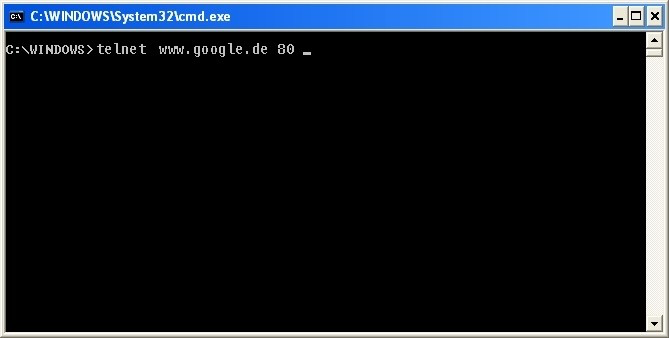
\includegraphics[width=.8\textwidth]{Q2-GK-AB.II.5-Abb_cmd.png}
\end{center}

Nun werden \textbf{alle} Eingaben (bei betätigen von \taste{ENTER}) an den Server geschickt. Alle Eingaben heißt, dass auch Tasten wie \taste{Backspace}, oder \taste{$\leftarrow$} (\appfunktion{Pfeil links}) übertragen werden. Die Eingabe

\begin{verbatim}
	HELLO
\end{verbatim}

ist also etwas anderes als die Eingabe

\begin{verbatim}
	HELLL<Backspace>O
\end{verbatim}

bei der man das überflüssige \enquote{L} vor dem abschicken wieder löscht. Manche Server können mit diesen \enquote{fehlerhaften} Eingaben umgehen, manche leider nicht.

Um eine Verbindung zu einem anderen Programm auf dem gleichen Rechner herzustellen kann die lokale IP \code{127.0.0.1} genutzt werden:

\begin{center}
	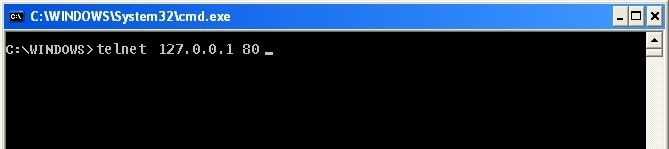
\includegraphics[width=.8\textwidth]{Q2-GK-AB.II.5-Abb_home.png}
\end{center}

\newpage

\begin{aufgabe}
Verbindet euch zu einem Webserver mit einem beliebigen Hostnamen (zum Beispiel \enquote{neugebauer.cc}, \enquote{ngb.schule}, \enquote{google.com} oder \enquote{whitehouse.gov}) und über den Port 80.

Ihr seid nun wie ein Browser mit dem Server verbunden und könnt über das \emph{HTTP-Protokoll} mit ihm kommunizieren. Die folgenden Befehlsfolge zeigt ein Beispiel, wie eine Webseite abgerufen werden kann:

\textbf{\code{telnet neugebauer.cc 80}}\\
{\color{gray}
\code{Trying 2a00:1158:1000:300::5f2...} \\
\code{Connected to neugebauer.cc.}\\ 
\verb|Escape character is '^]'.|
}

\textbf{\code{GET /index.html HTTP/1.1}} \\
\textbf{\code{host: neugebauer.cc}}

Informiert euch im Internet über das HTTP-Protokoll und besonders das GET-Kommando. Probiert dann verschiedene Kombinationen von Parametern für das GET-Kommando aus (versucht statt \enquote{/index.html} doch mal \enquote{/images/S4t.png} vom Host \enquote{neugebauer.cc} abzurufen).
\end{aufgabe}

\begin{aufgabe}
	Im Tauschordner findet ihr im Ordner \ordner{Server} verschiedene Server-Programme. Probiert sie aus, indem ihr eins startet und zum angezeigten Port verbindet:
	
	\code{telnet 127.0.0.1 <PORTNUMMER>}
	
	Probiert dann aus, verschiedene Nachrichten zu senden und herauszufinden, wie der Server funktioniert.
	
	\hinweis{Ihr könnt den Server auch auf einem anderen Rechner starten und statt zu \code{127.0.0.1} zur IP des Servers zu verbinden. Dazu müsst ihr auf der Server-Maschine zunächst die IP mit dem \code{ipconfig}-Kommando ermitteln.}
	
	\paragraph{Hinweise zum TicTacToe-Server:}
	Verbindet zum Port 1000: \code{telnet 127.0.0.1 1000}
	
	Es sind folgende Befehle erlaubt:
	
	\begin{tabularx}{\textwidth}{|l|X|}\hline
	\code{BOARD} & Zeigt das aktuelle Spielfeld und den Spielzustand an. \\\hline
	\code{RESTART} & Startet ein neues Spiel. \\\hline
	\code{NAME <name>} & Setzt zu Beginn den Nickname. \\\hline
	\code{SET <x>,<y>} & Setzt bei den Koordinaten (x | y) ein Kreuz. \\\hline
	\end{tabularx}

	Versucht ein Spiel komplett über \programm{telnet} zu spielen.
\end{aufgabe}

\begin{aufgabe}
	Wird kein Port angegeben, wird standardmäßig der Port 23 benutzt. Eine Verbindung kann entweder mit einem der Kommandos \code{exit} oder \code{quit} beendet werden, oder mit der Tastenkombination \keys{Strg+C} abgbrochen werden.
	
	Probiert \programm{telnet} Verbindungen zu einigen der folgenden Servern aus:
	
	\begin{itemize}
		\item \enquote{telehack.com} (Probiert dann das Kommando \code{eliza} aus. \code{help} erklärt euch die verfügbaren Kommandos.)
		\item \enquote{rainmaker.wunderground.com}
		\item  \enquote{towel.blinkenlights.nl} (Viel Spaß, aber bitte nicht bis zum Ende anschauen ;-) )
		\item \enquote{aardmud.org} oder \enquote{zombiemud.org} (siehe letzten Hinweis ...)
		\item \enquote{freechess.org}
		\item \enquote{mtrek.com} (Port 1701)
	\end{itemize}
\end{aufgabe}

\end{document}
